\chapter{Implementation details}
\label{cha:implementation}

Software engineering decisions, problems/solutions and resignations will be discussed in this chapter.

\section{Software engineering decisions}

\subsection{Why to re-implement the calibration estimation package?}

Willow Garage has a calibration package already implemented for calibration:

\url{http://www.ros.org/wiki/calibration}

\noindent
It is more generic package, it is able to calibrate the joint angles and different types of sensors all together.


\noindent
My code is a github fork of this repository:

\url{https://github.com/pablospe/calibration}

\noindent
Then, why re-implement it? A number of points: % was desired: % and the original package does not has:
\begin{itemize*}
 \item Easy to reuse for new robots.
 \item More speed.
 \item Pass to C++ (mainly for Ceres), before implemented in Python.
 \item The old calibration package uses DH parameters\footnote{The Denavit-Hartenberg parameters (DH parameters) are the four parameters associated with a particular convention for attaching reference frames to the links of a spatial kinematic chain, or robot manipulator.}, which has some problems with certain robots.
\end{itemize*}

Mainly for these points the decision to start from scratch the estimation part was taken.



\subsection{Why KDL?}

As is mentioned above, the old package uses DH parameters and it has its own kinematic library, instead of using the well tested KDL. Not only provides forward kinematic, it is also was useful for geometrics frame transformation, and conversion between different kind of rotation matrix parametrization (mainly between quaternions and angle-axis).



\subsection{Why to re-implement \texttt{robot\_state\_publisher}?}

\texttt{robot\_state\_publisher} is a package in ROS which publishes the state of a robot to \texttt{/tf}. It takes the joint angles of the robot as input and publishes the 3D poses of the robot links, using a kinematic tree model of the robot (KDL tree which is obtained from the URDF description).

There are 2 problems with this package:
\begin{itemize*}
 \item It does not allow to modify the URDF without constructing a new \texttt{robot\_state\_publisher} from the tree model. Note the important of this because the main goal of calibration is to update the URDF. In addition, since it is an optimization process and it must as fast as possible, it was not desired to send/receive messages during that stage.

 \item Another problem is that the fixed joints (non-mobile joints) are publish half a second later (for some unknown reason), and when the URDF is updated estrange behavior can occur.
\end{itemize*}

%
% Why KDL? KDL structures are not modificable, so it was needed to re-create KDL once the urdf is updated.
%
% RViz and Markers! Republish everytime!
%
% * Quaternions: used to avoid singularities...
%
% * Data/Views in different order... explain... some views aren't visible for all the cameras.
%
% (optional)
% Why Ceres?

\subsection{Quaternions}

One important observation is the use of quaternions. This decision was taken to avoid singularities that others rotation parametrization may have.

\newpage
\section{Code}
\subsection{Cost function}
\label{sec:ceres_impl}

The Ceres Solver cost function implemented is simple, mainly because distortion is not needed to be considered, since the images are already rectified.

\begin{lstlisting}[language=C++, label=code:cost_function, caption={Cost function}]
template <typename T>
void calc_residuals(double observed_x, double observed_y,
                    double fx, double fy, double cx, double cy,
                    const T* const camera_rotation,
                    const T* const camera_translation,
                    const T* const point,
                    T residuals[2])
{
  // camera_rotation are the quaternions
  T p[3];
  ceres::QuaternionRotatePoint(camera_rotation, point, p);

  // camera_translation is the translation
  p[0] += camera_translation[0];
  p[1] += camera_translation[1];
  p[2] += camera_translation[2];

  // Compute the projection
  T xp = p[0] / p[2];
  T yp = p[1] / p[2];
  T predicted_x = T(fx) * xp + T(cx);
  T predicted_y = T(fy) * yp + T(cy);

  // The error is the difference between the predicted and observed position.
  residuals[0] = predicted_x - T(observed_x);
  residuals[1] = predicted_y - T(observed_y);
}
\end{lstlisting}



\subsection{N-View Triangulation}
\label{sec:triangulation_impl}

This is a generalization of the triangulation method proposed in section \ref{sec:triangulation}.

\begin{lstlisting}[language=C++, label=code:triangulation, caption={Triangulation}]
// It is the standard DLT (for multiple views)
void nViewTriangulate(const Mat_<double> &x,
                      const vector<Matx34d> &Ps,
                      Vec3d &X)
{
  CV_Assert(x.rows == 2);
  unsigned nviews = x.cols;
  CV_Assert(nviews == Ps.size());

  cv::Mat_<double> design = cv::Mat_<double>::zeros(2 * nviews, 4);
  for (int i = 0; i < nviews; ++i) {
    for (int j = 0; j < 4; ++j) {
      design(i*2,   j) = x(0,i) * Ps[i](2, j) - Ps[i](0, j);
      design(i*2+1, j) = x(1,i) * Ps[i](2, j) - Ps[i](1, j);
    }
  }

  Mat X_homog;
  cv::SVD::solveZ(design, X_homog);
  homogeneousToEuclidean(X_homog, X);
}
\end{lstlisting}

% \section{...}

% \subsection{Creating model point for solvePnP}
% \label{sec:solvePnP_impl}
% It is was necessary to create a function that
%
% \begin{lstlisting}[language=C++, label=code:generateCorners, caption={generateCorners}]
% void ChessBoard::generateCorners(vector<Point3d> *corners)
% {
%   // clear corners
%   corners->clear();
%
%   // generate corners: (x,y,z)
%   for ( int j = 0; j < height_; j++ )
%     for ( int i = 0; i < width_; i++ )
%       corners->push_back( Point3d( float(i*square_size_),
%                                    float(j*square_size_), 0 ) );
% }
% \end{lstlisting}


\section{Problems and solutions}

\subsection{Visible cameras}

\textbf{Problem}: depending of the point of view, not all the checkerboards are visible for all the cameras (see Figure \ref{fig:visibility}). Moreover, the order of the cameras in the ROS messages can change. This complicated the whole process adding unexpected complexity to really simple tasks. It could have been avoided with a little of design.

\begin{figure}[!htbp]
 \centering
 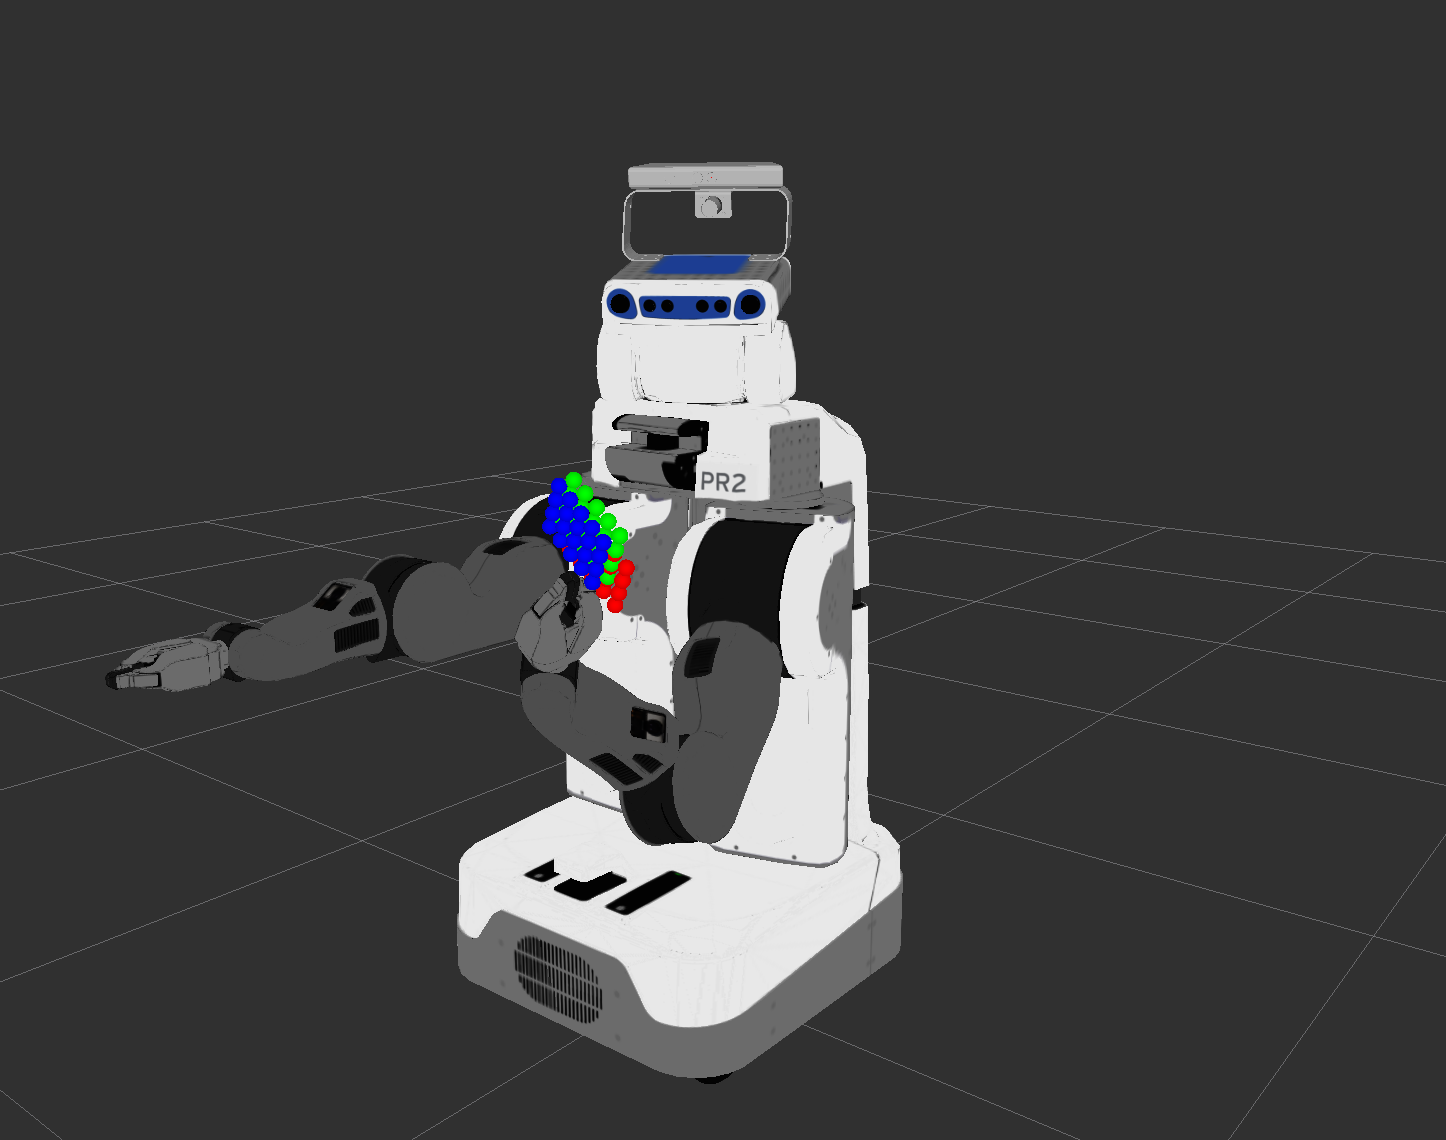
\includegraphics[width=0.45\textwidth]{images/screenshots/uncalib05.png}
 \caption{Checkerboard in hand visible only for 3 cameras.}
 \label{fig:visibility}
\end{figure}

\noindent
\textbf{Solution}: A class called \texttt{View} was created which works as a data container but in a well defined order. It has some ``mapping'' between cameras and frame names (coordinate system names).


\subsection{Robot update}

\textbf{Problem}: once the optimization process finishes, the result is not ready to be use. The rotation and translation matrices are relative to the first camera, and cannot be use to update the robot. A example in Figure \ref{fig:optimization_failer}, which was one of the initial ``solutions''.

\noindent
\textbf{Solution}: explanation given in section \ref{sec:update_urdf}.

\begin{figure}[!htbp]
 \centering
 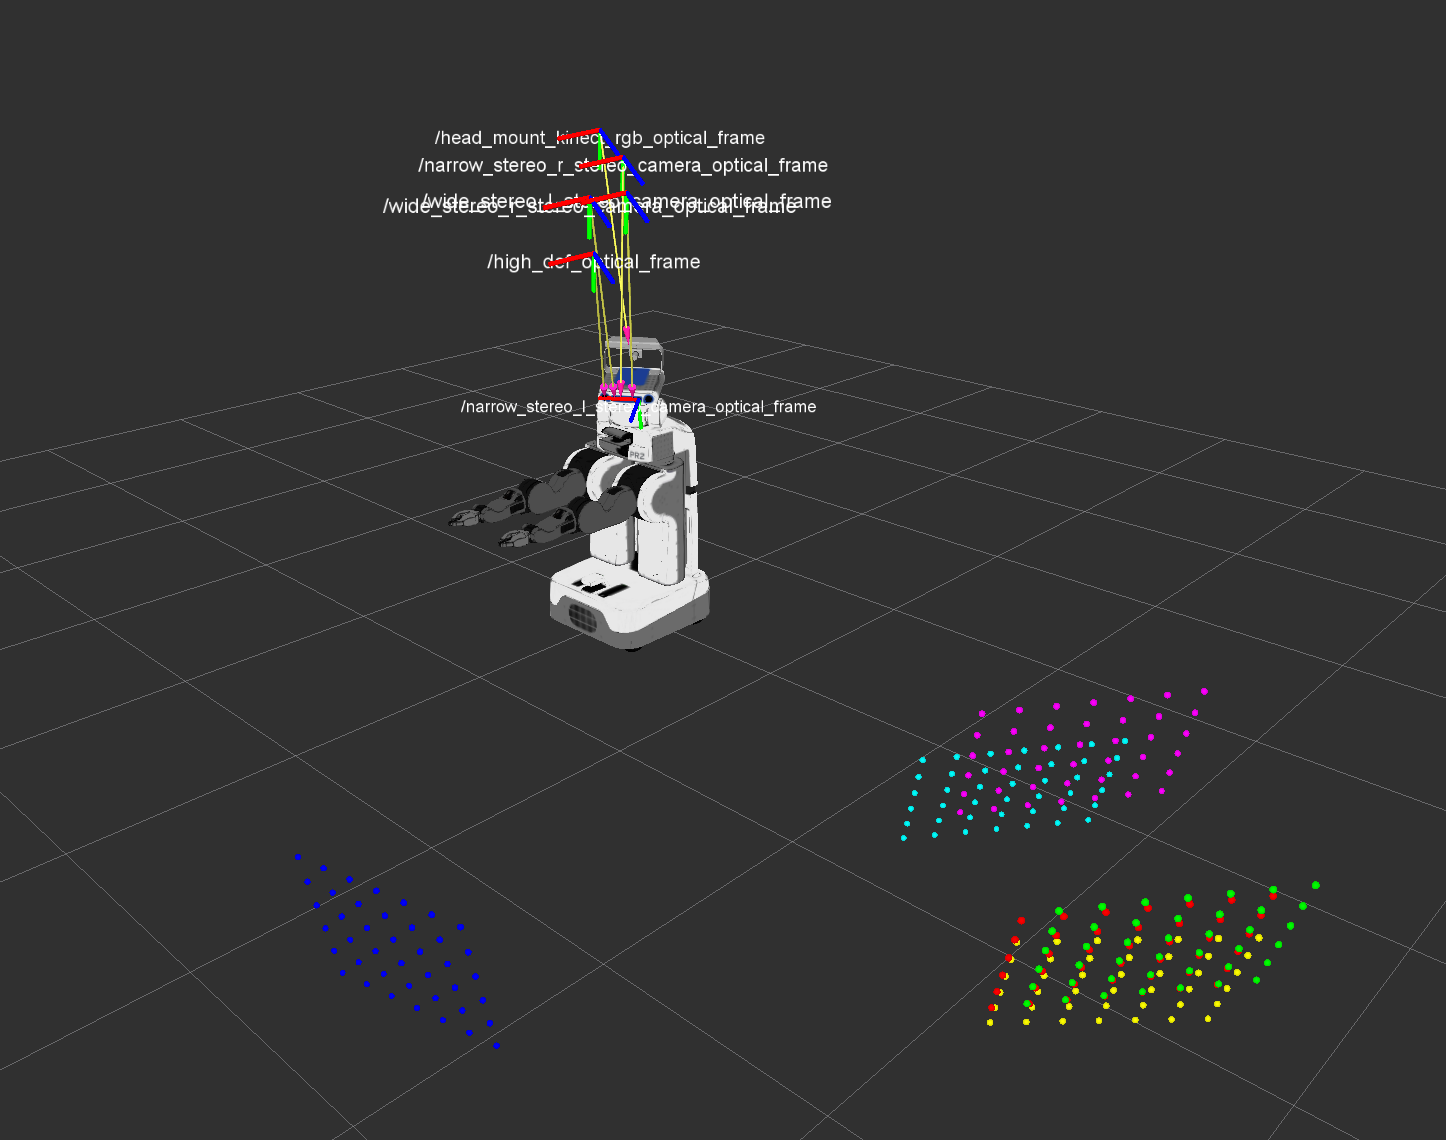
\includegraphics[width=0.55\textwidth]{images/screenshots/optimization_failer02_2.png}
 \caption{Initial versions}
 \label{fig:optimization_failer}
\end{figure}


\subsection{Multi-view triangulation}

\textbf{Problem}: Multi-view triangulation fails, see Figure \ref{fig:triangulation_fails}.

\noindent
\textbf{Solution}: no solution has been found by the moment of writing this thesis, the algorithm seems to be correct.

\begin{figure}[!htbp]
 \centering
 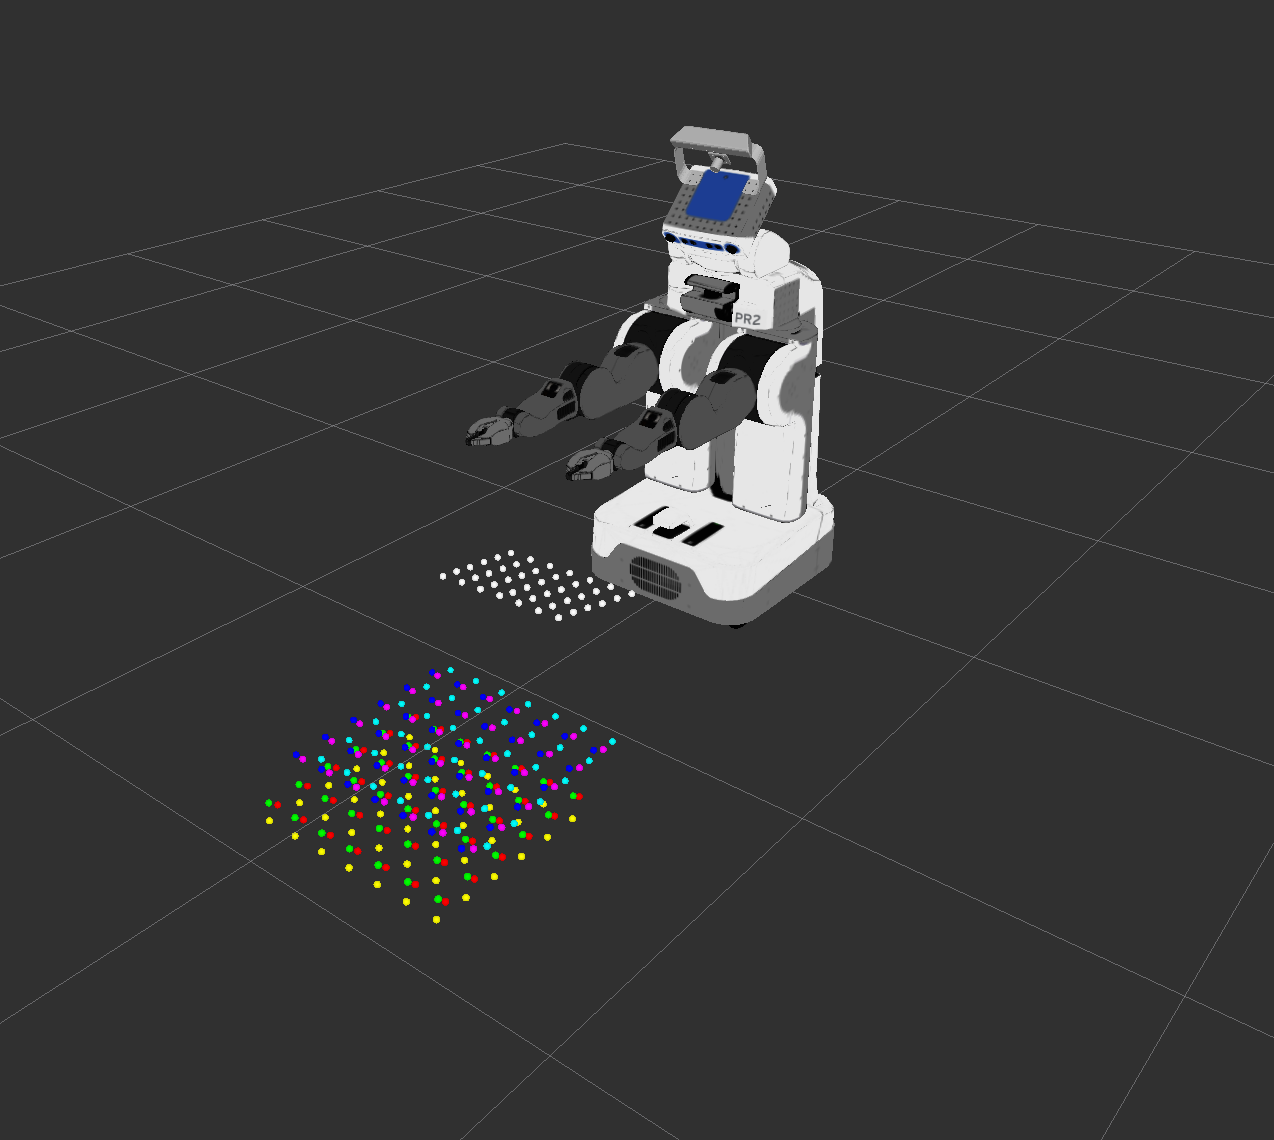
\includegraphics[width=0.55\textwidth]{images/screenshots/triangulation_fails.png}
 \caption{Triangulation fails, white dots}
 \label{fig:triangulation_fails}
\end{figure}

\vspace*{-2ex}
\section{Stats}
Just for fun, it took me 9,061 additions and 3,954 deletions in 99 commits until this point.
\begin{figure}[!htbp]
 \centering
 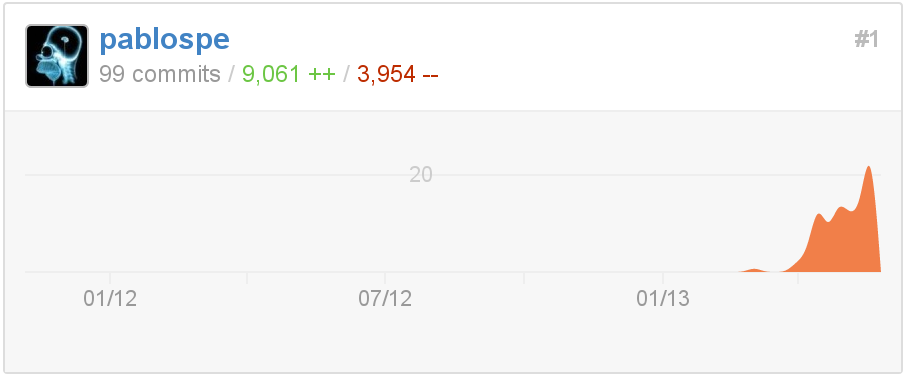
\includegraphics[width=0.65\textwidth]{images/git_stats.png}
 \caption{Github stats}
 \label{fig:triangulation_fails}
\end{figure}

Github repository: \url{https://github.com/pablospe/calibration}.

% \chapter{Extra work}
% \label{cha:extra}
%
% (this chapter is more than optional)
%
% Work not related to the thesis, but time consuming, like commits in Ceres, fixed bugs in URDF dom (export\_urdf() function), etc...

